\frame
{
\frametitle{Infraestructura}
\framesubtitle{\oran{Data Center}}
\begin{figure}
	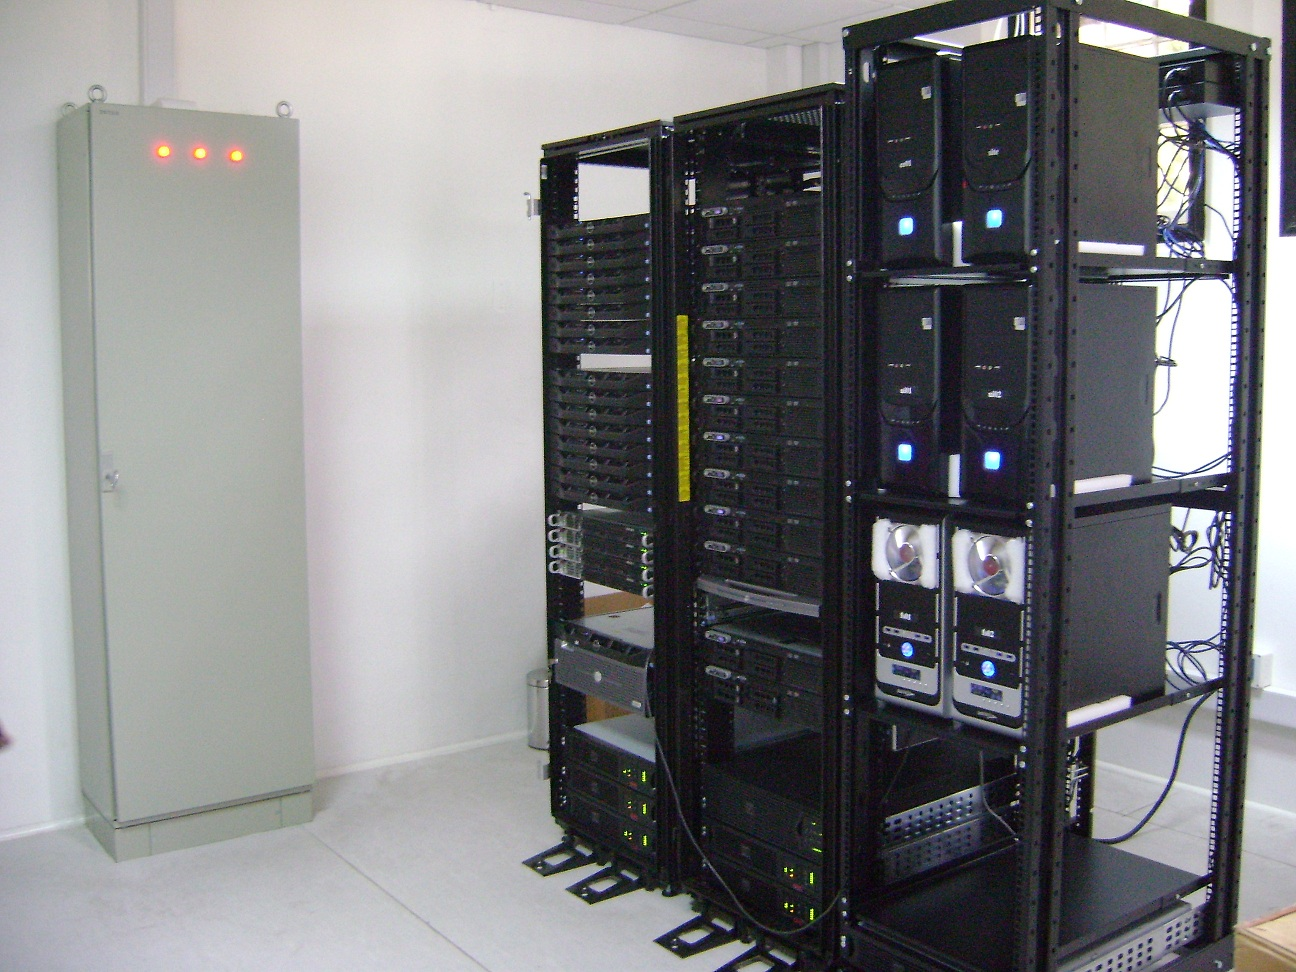
\includegraphics[scale=0.8]{img/cti_hpc_data_center}
\end{figure}
}


\frame
{
\frametitle{Infraestructura}
\framesubtitle{\oran{Data Center}}
El Data Center cuenta con 2 \emph{clusters}, y 4 Nodos GPU con las siguientes características:
\begin{table}[h]
\centering
\scalebox{0.65}{
	\begin{tabular}{|c|l|l|l|}
		\hline
						 & \textbf{Cluster 1} 		& \textbf{Cluster 2}		& \textbf{Nodos GPU} 	\\
		\hline
		\textbf{Nodes} 		 	&12				&16				&4			\\
		\hline
		\textbf{CPU}		 	&Dual Xeon 5110 1.60 GHz	&Dual Xeon X5560 2.8 GHz	&Dual Xeon E5520 2.27GHz\\
		\hline
		\textbf{Physical Cores}		&24 				&128				&1376			\\
		\hline
		\textbf{Logical Cores}		&48 				&256				&1376			\\
		\hline
		\textbf{RAM}		 	&4GB				&16GB				&24GB			\\
		\hline
		\textbf{Storage}	 	&12TB				&48TB				&250GB			\\
		\hline
		\textbf{GPU}		 	&-				&-				&Tesla M2050, C1060	\\
		\hline
	\end{tabular}}
\caption{Características de los equipos}
\end{table}
}

\frame
{
\frametitle{Infraestructura}
\framesubtitle{\oran{Hacia donde vamos}}
\begin{itemize}
\item Se busca pasar de \emph{Tier-III} a \emph{Tier-II} en proyecto ATLAS.

\item En los próximos meses se instalará un nuevo Cluster parte del proyecto NLHPC, 
que cuenta con las siguientes características.

\end{itemize}
\begin{table}[h]
\centering
\scalebox{0.8}{
	\begin{tabular}{|c|l|}
		\hline
					 & \textbf{Cluster Proyecto NLHPC} 	\\
		\hline
		\textbf{Nodos} 		 &12					\\			
		\hline
		\textbf{CPU}		 &Dual Xeon X5675 3.06GHz		\\
		\hline
		\textbf{Physical Cores}  &144					\\
		\hline
		\textbf{Logical Cores}	 &288					\\
		\hline
		\textbf{RAM}		 &32GB					\\
		\hline
		\textbf{Storage}	 &48TB					\\
		\hline
	\end{tabular}}
\caption{Características del Cluster Proyecto NLHPC}
\end{table}

}
